\documentclass[11pt]{beamer}
%\setbeamercovered{transparent}
\usepackage[utf8]{inputenc}
\usepackage[T1]{fontenc}
\usepackage{xeCJK} % this requires XeLaTeX
\setCJKmainfont{SimSun} % this correctly renders Japanese text
\usepackage{lmodern}
\usepackage{verbatim}
\usepackage{tikz}
\usepackage{amsmath, amsfonts, amssymb, amsthm, physics, mathtools, setspace, stmaryrd, stackrel, bbm, ifthen, commath,graphicx, hyperref}
\usetikzlibrary{trees, automata, positioning}
\usetheme{darmstadt}

\graphicspath{{./images/}}

\title{Aspect-Based Sentiment Analysis of Japanese Hotel Reviews}
\author{Tan Wei Chiong}
\date{February 28, 2024}

\begin{document}
	\begin{frame}[plain]
		\maketitle
	\end{frame}
	
	\begin{frame}[plain]
		\tableofcontents
	\end{frame}
	
	\section{Introduction}
	
	\begin{frame}
		\frametitle{Motivation}
		\begin{figure}
			\begin{center}
				\includegraphics[scale=0.25]{japanese_llm}
			\end{center}
			\caption{(Source: The Decoder. \url{https://the-decoder.com/japan-develops-its-own-culturally-sensitive-language-model/})}
		\end{figure}
	\end{frame}
	
	\begin{frame}
		\frametitle{Problem Statement}
		\begin{itemize}
			\item A hotel chain owner who mainly caters to Japanese tourists wants to find out how good or bad of an experience tourists had during their stay in the hotel.
			\pause
			\item However, many Japanese do not know enough English to leave a review without using an automatic translator application, and are much more comfortable leaving reviews in their native Japanese.
			\pause
			\item As a non-Japanese small business owner, it would be a great help to have a data-driven tool that can help to interpret their true sentiments about your service.
		\end{itemize}
	\end{frame}
	
	\begin{frame}
		\frametitle{Project Scope}
		\begin{itemize}
			\item Disclaimer: This is just a proof of concept.
			\pause
			\item Provide a brief introduction to Japanese NLP methods and tools.
			\pause
			\item Briefly compare two Japanese sentiment analyzers -- oseti and asari.
		\end{itemize}
	\end{frame}
		
	\section{Data Processing}
	
	\begin{frame}
		\frametitle{Data Source}
		\begin{center}
			\includegraphics[scale=0.6]{rt_logo}
		\end{center}
	\end{frame}
	
	\begin{frame}
		\frametitle{Why The Japanese Website Is Better For Scraping}
		\begin{itemize}
			\item Non-dynamic webpage -- easier access to relevant information;
			\pause
			\item Tends to be cluttered, but does not matter much to a scraper.
			\pause
			\item All reviews need to have the actual review text; the English site does not require that.
		\end{itemize}
	\end{frame}
	
	\begin{frame}
		\frametitle{Final Dataset}
		\begin{itemize}
			\item 7340 reviews total, from 182 hotels across the 6 prefectures of the Tohoku region:\\
			(Akita, Aomori, Fukushima, Iwate, Miyagi, Yamagata);
			\pause
			\item Reviews without ratings are ignored by the scraper;
			\pause
			\item 5568 reviews have all scores populated; this is used mainly for performance metrics.
		\end{itemize}
	\end{frame}
	
	\begin{frame}
		\frametitle{Data Workflow}
		\begin{center}
			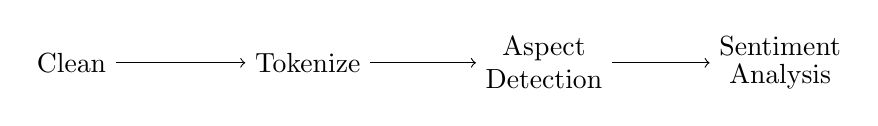
\begin{tikzpicture}
				\node (step1) at (-4,0) {Clean};
				\node (step2) at (-1,0) {Tokenize};
				\node (step3) at (2,0) {\shortstack{Aspect \\ Detection}};
				\node (step4) at (5,0) {\shortstack{Sentiment \\ Analysis}};
				
				\draw[->] (step1) -- (step2);
				\draw[->] (step2) -- (step3);
				\draw[->] (step3) -- (step4);
			\end{tikzpicture}
		\end{center}
	\end{frame}
	
	\begin{frame}
		\frametitle{Tokenization}
		Let's try to tokenize a sentence in English!
		\pause
		\begin{center}
			The reception was very polite.
		\end{center}
		\pause
		Easy? What about a Japanese sentence? 
		\pause
		\begin{center}
			フロントはとても丁寧でした。
		\end{center}
	\end{frame}
	
	\begin{frame}
		\frametitle{Japanese Language 101 -- Hiragana}
		\begin{center}
			\textcolor{lightgray}{フロント} は\ とても \textcolor{lightgray}{丁寧} でした。
		\end{center}
		\pause
		\begin{itemize}
			\item Basic alphabet of Japanese;
			\pause
			\item Used for particles;
			\pause
			\item Used for words without kanji representation.
		\end{itemize}
	\end{frame}
	
	\begin{frame}
		\frametitle{Japanese Language 101 -- Katakana}
		\begin{center}
			フロント \textcolor{lightgray}{は\ とても\ 丁寧\ でした。}
		\end{center}
		\pause
		\begin{itemize}
			\item Same pronunciations as hiragana, different script;
			\pause
			\item Used for loan words.
		\end{itemize}
	\end{frame}
	
	\begin{frame}
		\frametitle{Japanese Language 101 -- Kanji}
		\begin{center}
			\textcolor{lightgray}{フロント\ は\ とても} 丁寧 \textcolor{lightgray}{でした。}
		\end{center}
		\pause
		\begin{itemize}
			\item Originated from the Chinese script;
			\item Each kanji has at least 2 pronunciations -- kun-yomi (Japanese pronunciation) and on-yomi (Chinese pronunciation);
			\item Provides semantics to words.
		\end{itemize}
	\end{frame}
	
	\begin{frame}
		\frametitle{Different Tools for a Different Context}
		\begin{itemize}
			\item We cannot simply tokenize based on spaces, because word boundaries are not that clear!
			\pause
			\item Lattice-based tokenization is needed.
		\end{itemize}
	\end{frame}
	
	\begin{frame}
		\frametitle{Lattice-based Tokenization}
		\begin{itemize}
			\item Each connection has an associated cost;
			\item The most probable tokenization is the route with the lowest total cost.\\
		\end{itemize}
		\begin{figure}
			\includegraphics[scale=0.5]{japanese_tokenization}
			\caption{A lattice of tokens (Credit: Wanasit Tanakitrungruang)}
		\end{figure}
	\end{frame}
	
	\begin{frame}
		\frametitle{Our Chosen Tokenizer}
		A widely-used dictionary for Japanese tokenization is MeCab, written in C++.\\
		\pause
		\begin{figure}
			\begin{center}
				\includegraphics[scale=0.2]{mekabu}
			\end{center}
			\caption{Mekabu (Source: Wakasa no Himitsu)}
		\end{figure}
	\end{frame}
	
	\begin{frame}
		\frametitle{Our Chosen Tokenizer}
		We shall use natto-py, self-described as ``A Tasty Python Binding with MeCab''.\\
		\pause
		\begin{figure}
			\begin{center}
				\includegraphics[scale=0.3]{natto_on_rice}
			\end{center}
			\caption{Natto on rice. (Source: Wikipedia)}
		\end{figure}
	\end{frame}
	
	\begin{frame}
		\frametitle{Aspect Detection}
		\begin{itemize}
			\item We use natto-py together with CountVectorizer to extract out a list of the most common words in the entire dataset;
			\item Then assign each sentence in a review its relevant aspects.
		\end{itemize}
	\end{frame}
	
	\begin{frame}
		\frametitle{Example output for natto-py}
		A token from natto-py looks like: \begin{center}
			良かっ,	形容詞,非自立,*,*,形容詞アウオ段,連用タ接続,良い,ヨカッ,ヨカッ
		\end{center}
		\pause
		In English, a similar tokenization would look something like: \begin{center}
			running,	verb,*,*,*,*,present progressive tense,run,run,run
		\end{center}
	\end{frame}
	
	\begin{frame}[allowframebreaks]
		\frametitle{Aspect Keywords}
		\begin{table}
			{\renewcommand{\arraystretch}{1.5}
				\renewcommand{\tabcolsep}{0.2cm}
				\begin{tabular}{|p{0.15\linewidth}|p{0.35\linewidth}|p{0.45\linewidth}|}
					\hline
					Aspect & Definition & Keywords\\
					\hline
					Service & Acts of help towards customer satisfaction & サービス, スタッフ, フロント, チェックイン, 丁寧, 親切, 接客, サーバ\\
					\hline
					Location & Access and landscape around the hotel & 立地, 駅, バス, 近く, 便利, 駐車, コンビニ, 場所\\
					\hline
					Room & The attributes of the room & 部屋, 広い, 宿泊, ベッド, 値段\\
					\hline
			\end{tabular}}
		\end{table}
		
		\begin{table}
			{\renewcommand{\arraystretch}{1.5}
			\renewcommand{\tabcolsep}{0.2cm}
			\begin{tabular}{|p{0.15\linewidth}|p{0.35\linewidth}|p{0.45\linewidth}|}
				\hline
				Aspect & Definition & Keywords\\
				\hline
				Amenities & Other facilities in the hotel excluding room and bath & アメニティ, 無料\\
				\hline
				Bathroom & Bath in the hotel room, or a public bath & 風呂, 温泉, 浴場, 露天風呂, 清潔, 湯, トイレ\\
				\hline
				Food & Morning or evening meals & 朝食, 食事, 料理, 夕食, バイキング, メニュー, ご飯, 酒, 飲\\
				\hline
			\end{tabular}}
		\end{table}
	\end{frame}
	
	\begin{frame}
		\frametitle{Example: Aspect Identification in a Review}
		\begin{description}
			\item[Review:] ``日本酒の飲み比べサーバは良かったです。また、部屋もきれいでスマホ充電など細かな気遣いも良かったです''
			\pause
			\item[Translation:] ``The server for the Japanese sake tasting was good. Likewise, the room was clean, and it was good that there was little to worry about things like smartphone chargers, etc.\@ as well''
			\pause
			\item[Aspects:] 
			\begin{description}
				\item[Service:] ``日本酒の飲み比べ\textcolor{red}{サーバ}は良かったです''
				\item[Food:] ``日本\textcolor{red}{酒}の\textcolor{red}{飲}み比べサーバは良かったです''
				\item[Room:] ``また、\textcolor{red}{部屋}もきれいでスマホ充電など細かな気遣いも良かったです''
			\end{description}
		\end{description}
	\end{frame}
	
	\section{Modelling}
	
	\begin{frame}
		\frametitle{oseti -- A Japanese Sentiment Analysis Tool}
		\begin{itemize}
			\item Dictionary-based -- relevant words are matched with their sentiment polarity in a dictionary (positive, negative);
			\pause
			\item Text is analyzed at the sentence level; the overall sentiment is a simple weighted sum of positive and negative token sentiments;
			\pause
			\item Does not consider position of words in a sentence.
		\end{itemize}
		\pause
		\begin{figure}
			\begin{center}
				\includegraphics[scale=0.25]{oseti}
			\end{center}
			\caption{A Japanese \textit{oseti} (Source: Wikipedia)}
		\end{figure}
	\end{frame}
	
	\begin{frame}
		\frametitle{asari -- Another Japanese Sentiment Analysis Tool}
		\begin{figure}
			\begin{center}
				\includegraphics[scale=0.4]{behold_asari}
			\end{center}
			\caption{Documentation for asari}
		\end{figure}
	\end{frame}
	
	\begin{frame}
		\frametitle{asari -- Another Japanese Sentiment Analysis Tool}
		\begin{itemize}
			\item Trained using a Linear Support Vector Classifier;
			\pause
			\item Returns the positive and negative sentiments as probabilities (confidence levels).
		\end{itemize}
		\pause
		\begin{figure}
			\begin{center}
				\includegraphics[scale=0.13]{asari_udon}
			\end{center}
			\caption{Asari clams with udon (Source: Wikipedia)}
		\end{figure}
	\end{frame}
	
	\begin{frame}
		\frametitle{Sentiment Analysis Methodology}
		\begin{enumerate}
			\item We take each of the aspects contained in the review, and assign two sentiment scores using oseti and asari respectively (per aspect);
			\pause
			\item Convert each sentiment score (a number from -1 to 1) into a rating from 1 to 5;
			\pause
			\item The ratings given by the customer for their reviews will be taken as a ``ground truth'', and the predicted scores will be compared against them.
		\end{enumerate}
	\end{frame}
	
	\begin{frame}
		\frametitle{Example Analysis of Review}
		Let's look at the ``food'' aspect of the following review: \begin{flushleft}
			家族でのんびり過ごせて良かったです。お料理が美味しかったし、景色も美しかったです。温泉は思ったよりも小さかったですが、泉質は結構よかった。
		\end{flushleft}
		Translated, it reads: \begin{flushleft}
			I had a relaxing stay with my family. The food was delicious, and the scenery was beautiful too. Though the hot spring was smaller than I thought, the spring water was rather good.
		\end{flushleft}
		\pause
		\begin{table}
			\begin{tabular}{|c|c|c|}
				\hline
				Analyzer & Sentiment & Predicted Score\\
				\hline
				oseti & 1 & 5\\
				\hline
				asari & 0.887214 & 5\\
				\hline
			\end{tabular}
		\end{table}
	\end{frame}
	
	\begin{frame}
		\frametitle{Model Evaluation}
		As classifiers, neither sentiment analyzer performs well.
		
		However, a prediction of 4 stars when the actual customer rates 5 stars is still not too bad.
		\pause
		
		Thus, we use the \emph{mean absolute error} as a metric to gauge the performance of both models.
	\end{frame}
	
	\begin{frame}
		\begin{figure}
			\begin{center}
				\includegraphics[scale=0.25]{sentiments_graph}
			\end{center}
			\caption{Plot of sentiments and ratings}
		\end{figure}
	\end{frame}
	
	\begin{frame}
		\frametitle{Aspect-Based Comparison of Mean Absolute Errors}
		\begin{table}
			\begin{center}
				{\renewcommand{\arraystretch}{1.5}
					\renewcommand{\tabcolsep}{0.2cm}
					\begin{tabular}{|r|c|c|}
						\hline
						& oseti & asari\\
						\hline
						Overall & 0.836027 & 0.600395\\
						\hline
						Service & 1.054956 & 1.008441\\
						\hline
						Location & 1.183908 & 1.095725\\
						\hline
						Room & 1.072557 & 0.953125\\
						\hline
						Amenities & 1.086745 & 1.084590\\
						\hline
						Bathroom & 0.943426 & 0.839260\\
						\hline
						Food & 0.947198 & 0.795617\\
						\hline
				\end{tabular}}
			\end{center}
		\end{table}
	\end{frame}
	
	\section{Limitations and Future Work}
	
	\begin{frame}
		\frametitle{Limitations}
		\begin{itemize}
			\item More time, more data;
			\pause
			\item Proper labelling of aspects;
			\pause
			\item Accounting for zero anaphora; 選んでいただいたものなら何でも結構です。 (\textit{erande itadaita mono nara nandemo kekkou desu}, lit. ``Whatever (you) pick is fine.'') -- aspects may not appear even though the customer intended it.
		\end{itemize}
	\end{frame}
	
	\begin{frame}
		\frametitle{Future Work}
		\begin{itemize}
			\item Collecting data from all prefectures of Japan, perhaps from other countries as well;
			\pause
			\item Utilize a neural network approach to find hidden meanings;
			\pause
			\item Work out a translation scheme that keeps the intent as accurately as possible.
		\end{itemize}
	\end{frame}
	
	\begin{frame}
		\frametitle{Summary}
		\tableofcontents
	\end{frame}
	
	\begin{frame}
		\frametitle{The End}
		Thank you.
	\end{frame}
	
\end{document}